\subsection{OHD and Balanced-OHD Pattern Selection}

The previous sections described how OTFS-IM uses an activation-pattern table to map index bits into active delay-Doppler positions. This section focuses on how that table is selected. In the original OTFS-IM structure, any subset of valid constant-weight activation patterns can be used as long as the number of selected patterns is \(2^{b_1}\). However, different pattern tables do not necessarily have the same detection reliability. If two patterns are very similar, a small detection error in one position may cause the receiver to select the wrong index pattern. Therefore, pattern-table design becomes an important part of the implemented OTFS-IM system.

In this thesis, two deterministic selection rules are considered. The first one is the OHD method, which selects patterns with the largest minimum Hamming distance. The second one is Balanced-OHD, denoted as B-OHD, which keeps the same primary OHD objective but adds tie-breaking criteria related to average distance and carrier-usage balance.

\subsubsection{Pattern-Selection Problem Formulation}

For an IM block of length \(n\) with \(k\) active positions, the full set of constant-weight patterns is
\begin{equation}
    \mathcal{C}
    =
    \left\{
    \mathbf{p} \subset \{1,2,\ldots,n\}
    \; \middle| \;
    |\mathbf{p}| = k
    \right\}.
    \label{eq:full_pattern_candidate_set}
\end{equation}
The number of candidates is
\begin{equation}
    |\mathcal{C}|
    =
    \binom{n}{k}.
    \label{eq:number_of_candidate_patterns}
\end{equation}
Each candidate pattern contains the active local positions of one IM block. The complete set can be generated by enumerating all \(k\)-element subsets of \(\{1,2,\ldots,n\}\).

Since only \(b_1=\lfloor \log_2 \binom{n}{k} \rfloor\) index bits are assigned to one IM block, the pattern table used for transmission contains
\begin{equation}
    L
    =
    2^{b_1}
    \label{eq:number_of_selected_patterns}
\end{equation}
patterns. The design problem is therefore to select a subset
\begin{equation}
    \mathcal{M}
    \subseteq
    \mathcal{C},
    \qquad
    |\mathcal{M}| = L,
    \label{eq:selected_pattern_subset}
\end{equation}
and store it as the selected pattern table \(\mathcal{P}_{\mathrm{sel}}\), which corresponds to the activation-pattern table \(\mathcal{P}\) used in the transmitter and receiver descriptions. This table maps index bits to active positions at the transmitter and restricts the block-wise MAP search to valid candidate patterns at the receiver.

To evaluate the separation between patterns, each pattern is represented by a binary vector of length \(n\). For a pattern \(\mathbf{p}_i\), its binary representation is denoted by \(\mathbf{a}_i\), where
\begin{equation}
    a_i(\ell)
    =
    \begin{cases}
    1, & \ell \in \mathbf{p}_i,\\
    0, & \ell \notin \mathbf{p}_i.
    \end{cases}
    \label{eq:binary_pattern_representation}
\end{equation}
The Hamming distance between two candidate patterns is then
\begin{equation}
    d_{\mathrm{H}}(\mathbf{p}_i,\mathbf{p}_j)
    =
    \sum_{\ell=1}^{n}
    a_i(\ell) \oplus a_j(\ell),
    \label{eq:ohd_pattern_hamming_distance}
\end{equation}
where \(\oplus\) denotes the exclusive-or operation. The resulting pairwise distances form the Hamming-distance matrix used during pattern-table selection.

\subsubsection{OHD Criterion Based on Hamming Distance}

The purpose of the OHD method is to select a pattern table whose closest pair of patterns is as far apart as possible. For a candidate table \(\mathcal{M}\), the minimum pairwise Hamming distance is
\begin{equation}
    d_{\min}(\mathcal{M})
    =
    \min_{\mathbf{p}_i,\mathbf{p}_j \in \mathcal{M},\, i\neq j}
    d_{\mathrm{H}}(\mathbf{p}_i,\mathbf{p}_j).
    \label{eq:pattern_minimum_hamming_distance}
\end{equation}
The OHD-selected table is obtained by
\begin{equation}
    \mathcal{M}_{\mathrm{OHD}}
    =
    \arg\max_{\mathcal{M}\subseteq\mathcal{C},\,|\mathcal{M}|=L}
    d_{\min}(\mathcal{M}).
    \label{eq:ohd_selection_rule}
\end{equation}
This criterion is simple but meaningful for OTFS-IM detection. If two selected activation patterns differ in many positions, then the receiver must make more position-level mistakes before confusing one pattern with the other. As a result, a larger \(d_{\min}\) is expected to reduce the pattern error rate and, consequently, the index BER.

For exact OHD selection, all candidate pattern subsets are enumerated when the search is computationally feasible. For each subset, the method computes its minimum pairwise Hamming distance and keeps the subset with the largest value. The selected table is then used as the activation-pattern table, while diagnostic quantities such as minimum distance, distance matrix, and balance metrics are retained for analysis.

The OHD rule should be interpreted as a geometry-based table design method rather than a detector modification. It does not change the OTFS modulator, the channel model, or the MP detector equations. Instead, it changes which activation patterns are allowed to represent index bits. This distinction is important for the simulation analysis in Chapter 5, because any performance difference between OHD OTFS-IM and another OTFS-IM pattern table can be traced back to the pattern geometry.

\subsubsection{Balanced-OHD Tie-Breaking Strategy}

In many IM configurations, several candidate pattern tables can have the same maximum minimum Hamming distance. The pure OHD method only guarantees the best value of \(d_{\min}\), but it does not necessarily distinguish between tables that are tied under this primary criterion. Balanced-OHD addresses this limitation by keeping the OHD objective as the first priority and then applying additional tie-breaking rules.

For a selected table \(\mathcal{M}\), the average pairwise Hamming distance is defined as
\begin{equation}
    \bar{d}_{\mathrm{H}}(\mathcal{M})
    =
    \frac{2}{L(L-1)}
    \sum_{i<j}
    d_{\mathrm{H}}(\mathbf{p}_i,\mathbf{p}_j).
    \label{eq:average_hamming_distance}
\end{equation}
The number of closest pairs is
\begin{equation}
    N_{\min}(\mathcal{M})
    =
    \left|
    \left\{
    (i,j): i<j,\,
    d_{\mathrm{H}}(\mathbf{p}_i,\mathbf{p}_j)=d_{\min}(\mathcal{M})
    \right\}
    \right|.
    \label{eq:number_of_minimum_distance_pairs}
\end{equation}
In addition, the carrier-usage vector is
\begin{equation}
    \mathbf{u}
    =
    \sum_{\mathbf{p}_i\in\mathcal{M}}
    \mathbf{a}_i,
    \label{eq:carrier_usage_vector}
\end{equation}
where \(u_\ell\) indicates how many selected patterns use the \(\ell\)-th local position. The implemented balance metrics are
\begin{equation}
    J_{\mathrm{var}}
    =
    \sum_{\ell=1}^{n}
    \left(u_\ell-\bar{u}\right)^2,
    \qquad
    J_{\mathrm{span}}
    =
    \max_\ell u_\ell - \min_\ell u_\ell.
    \label{eq:carrier_usage_balance_metrics}
\end{equation}

The B-OHD method ranks candidate pattern tables in lexicographic order. The first priority is to maximize \(d_{\min}\). If two tables have the same \(d_{\min}\), the method selects the one with larger \(\bar{d}_{\mathrm{H}}\). If the tie still remains, it selects the table with fewer closest pairs \(N_{\min}\). Finally, if the distance statistics are still identical, it chooses the table with smaller carrier-usage variance and smaller carrier-usage span.

Therefore, B-OHD can be expressed conceptually as
\begin{equation}
    \mathcal{M}_{\mathrm{B\text{-}OHD}}
    =
    \arg\operatorname{best}_{\mathcal{M}}
    \left(
    d_{\min},
    \bar{d}_{\mathrm{H}},
    -N_{\min},
    -J_{\mathrm{var}},
    -J_{\mathrm{span}}
    \right).
    \label{eq:balanced_ohd_selection_rule}
\end{equation}
The signs in this expression indicate that larger distance metrics are preferred, while smaller closest-pair and imbalance metrics are preferred.

Figure~\ref{fig:ohd_balanced_pattern_selection_flow} summarizes the implemented OHD and B-OHD selection process.

\begin{figure}[H]
    \centering
    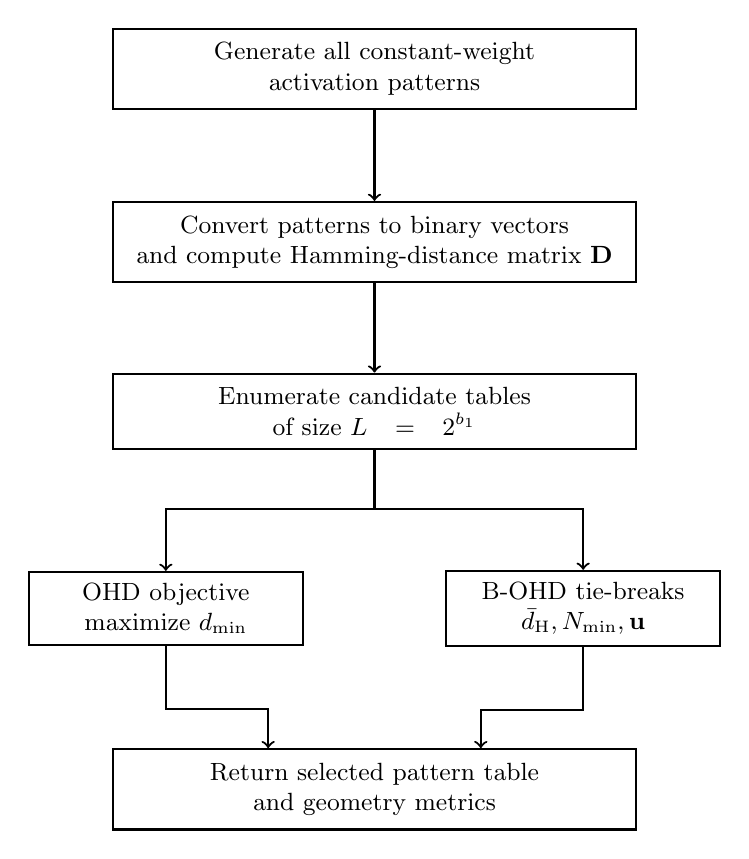
\begin{tikzpicture}[
        block/.style={
            rectangle,
            draw,
            thick,
            align=center,
            text width=6.3cm,
            minimum height=0.9cm,
            font=\small,
            inner sep=5pt
        },
        smallblock/.style={
            rectangle,
            draw,
            thick,
            align=center,
            text width=3.2cm,
            minimum height=0.85cm,
            font=\small,
            inner sep=4pt
        },
        arrow/.style={->, thick}
    ]

        \node[block] (all) at (0,0) {Generate all constant-weight\\activation patterns};
        \node[block] (bin) at (0,-2.20) {Convert patterns to binary vectors\\and compute Hamming-distance matrix \(\mathbf{D}\)};
        \node[block] (sets) at (0,-4.35) {Enumerate candidate tables\\of size \(L=2^{b_1}\)};
        \node[smallblock] (ohd) at (-2.65,-6.85) {OHD objective\\maximize \(d_{\min}\)};
        \node[smallblock] (bohd) at (2.65,-6.85) {B-OHD tie-breaks\\\(\bar{d}_{\mathrm{H}}, N_{\min}, \mathbf{u}\)};
        \node[block] (map) at (0,-9.15) {Return selected pattern table\\and geometry metrics};

        \draw[arrow] (all.south) -- (bin.north);
        \draw[arrow] (bin.south) -- (sets.north);
        \draw[arrow] (sets.south) -- ++(0,-0.75) -| (ohd.north);
        \draw[arrow] (sets.south) -- ++(0,-0.75) -| (bohd.north);
        \draw[arrow] (ohd.south) -- ++(0,-0.80) -| ([xshift=-1.35cm]map.north);
        \draw[arrow] (bohd.south) -- ++(0,-0.80) -| ([xshift=1.35cm]map.north);

    \end{tikzpicture}
    \caption{Pattern-selection flow for OHD and Balanced-OHD}
    \label{fig:ohd_balanced_pattern_selection_flow}
\end{figure}

The purpose of B-OHD is not to claim that carrier balance always dominates the pure OHD choice. Instead, it provides a controlled extension of OHD when multiple tables share the same minimum Hamming distance. This is why Chapter 5 reports OHD and B-OHD separately. If both methods select equivalent or nearly equivalent pattern tables for a given \((n,k)\), their BER curves may overlap. Such a result is not a failure of the method; it means that the selected pattern geometries are effectively the same under that configuration.

\subsubsection{Interpretation of the Pattern-Selection Outputs}

The pattern-selection stage produces more than the selected activation table. It also produces geometry indicators that help explain the BER results in Chapter 5. The most important indicator is \(d_{\min}\), because it describes the closest pair of patterns in the selected table. A larger \(d_{\min}\) generally means that a larger number of position-level mistakes is required before one valid index label can be confused with another.

The average Hamming distance \(\bar{d}_{\mathrm{H}}\) provides a complementary view. While \(d_{\min}\) focuses on the worst-separated pair, the average distance describes the overall separation of the selected table. Two tables can have the same \(d_{\min}\) but different average distances. In that case, B-OHD may prefer the table whose patterns are more separated on average, even if the worst-case pair is unchanged.

The number of closest pairs \(N_{\min}\) is also useful. If many pattern pairs achieve the minimum distance, the receiver has many vulnerable pattern confusions. If only one or two pairs are at the minimum distance, the weak part of the table is more localized. This distinction can affect the pattern error rate, especially at moderate SNR values where the MP probability map is informative but not yet fully reliable.

Finally, the carrier-usage vector \(\mathbf{u}\) indicates whether some local positions are used much more frequently than others. Strong imbalance is not always harmful by itself, but it may make the selected table less robust when certain positions have less reliable probability estimates. The balance metrics in B-OHD therefore serve as secondary tie-breakers, not as replacements for Hamming-distance separation.

\begin{table}[H]
\centering
\caption{Interpretation of pattern-selection criteria.}
\label{tab:pattern_selection_criteria_interpretation}
\begin{tabularx}{0.95\linewidth}{|p{3.2cm}|X|}
\hline
\textbf{Criterion} & \textbf{Interpretation in OTFS-IM detection} \\
\hline
\(d_{\min}\) & Worst-case separation between selected activation patterns; directly related to the most vulnerable pattern confusion. \\
\hline
\(\bar{d}_{\mathrm{H}}\) & Average geometric separation of the selected table; useful when several tables share the same \(d_{\min}\). \\
\hline
\(N_{\min}\) & Number of pattern pairs at the minimum distance; fewer closest pairs means fewer weakest confusions. \\
\hline
\(J_{\mathrm{var}}\), \(J_{\mathrm{span}}\) & Balance of local resource usage across the selected table; used only as secondary tie-breakers in B-OHD. \\
\hline
Random baseline & Diagnostic reference for checking whether deterministic table selection is actually beneficial. \\
\hline
\end{tabularx}
\end{table}

This interpretation is important because a lower total BER should not be attributed to OHD or B-OHD blindly. The selected table must also be examined through its geometry. If the selected tables have the same \(d_{\min}\), similar average distance, and similar carrier-usage statistics, then similar BER behavior is expected. Conversely, if one table has a clearly better distance profile, improvement in pattern error rate and index BER becomes more meaningful.

\subsubsection{Search Complexity and Random Diagnostic Baseline}

The exact OHD and B-OHD implementations enumerate all possible pattern tables of size \(L\) from \(\binom{n}{k}\) candidates. The number of candidate tables is
\begin{equation}
    N_{\mathrm{set}}
    =
    \binom{\binom{n}{k}}{L}.
    \label{eq:pattern_search_complexity}
\end{equation}
This search is acceptable for the small and moderate IM configurations used in this thesis, but it grows rapidly as \(n\) and \(k\) increase. For this reason, the implementation includes a guard condition that stops the exact search when the number of candidate tables exceeds a practical threshold. This keeps the simulation workflow focused on interpretable thesis configurations rather than on large-scale combinatorial optimization.

The simulation framework also includes a random-pattern diagnostic baseline. This baseline does not represent a proposed method. Its role is to test whether the deterministic pattern-selection rule provides a meaningful advantage over arbitrary valid pattern tables. In other words, random selection is used as an evaluation tool, not as a final design choice. If OHD or B-OHD gives lower pattern error rate and index BER than the random average, the result supports the claim that pattern geometry matters. If the random average is similar or better in some configurations, the result must be reported honestly and interpreted as a limitation of pure distance-based pattern selection for that configuration.

This distinction is important for the final evaluation. The baseline OTFS curve shows the effect of adding index modulation to OTFS. The OHD and B-OHD curves show the effect of deterministic pattern-table design inside OTFS-IM. The random-pattern curve, when enabled, checks whether the observed behavior is genuinely caused by the proposed table design or merely by the use of any valid activation-pattern subset.
